\section{Exact Dimension-Three Characterization}\label{sec:three}

We now specialize the simplex reduction to real \(3\times3\) matrices. Assume first that \(-A\) is a strict \(P\)-matrix and write
\[
p_i=-a_{ii}>0,\qquad
m_{12},m_{13},m_{23}>0,\qquad
q=-\det A>0,
\]
with the normalized invariants in Equation~\eqref{eq:four-invariants}. For
\[
D=\diag(d_1,d_2,d_3)\succ0
\]
the characteristic polynomial is
\begin{equation}
\det(\lambda I-DA)
=
\lambda^3+a_D\lambda^2+b_D\lambda+c_D,
\label{eq:cubicD}
\end{equation}
where
\begin{align}
a_D&=p_1d_1+p_2d_2+p_3d_3,\\
b_D&=m_{12}d_1d_2+m_{13}d_1d_3+m_{23}d_2d_3,\\
c_D&=q\,d_1d_2d_3.
\end{align}
With
\[
x_i=\frac{p_id_i}{a_D},
\qquad x\in\Delta_2^\circ,
\]
define
\begin{equation}
B_\beta(x)
=
\beta_{12}x_1x_2+
\beta_{13}x_1x_3+
\beta_{23}x_2x_3.
\label{eq:Bbeta}
\end{equation}
Then
\begin{equation}
\frac{b_D}{a_D^2}=B_\beta(x),
\qquad
\frac{c_D}{a_D^3}=\kappa x_1x_2x_3.
\label{eq:normalized-coeffs}
\end{equation}

\subsection{The Fixed-Cubic Matignon Boundary}

The fixed-polynomial component is a fractional Routh--Hurwitz/root-location problem; related coefficient-space criteria are established in the literature \cite{CermakNechvatal2017,BourafaAbdelouahabMoussaoui2020}. We state the exact form required for the diagonal-orbit elimination.

\begin{Lemma}[boundary value for a positive cubic]\label{lem:cubic-boundary}
Let
\[
p(\lambda)=\lambda^3+a\lambda^2+b\lambda+c,
\qquad a,b,c>0,
\]
and let
\[
\frac{\pi}{3}<\theta<\frac{\pi}{2}.
\]
Set
\[
u=\cos\theta,\qquad K=1-4u^2>0,
\]
and define
\begin{equation}
r_\theta(a,b)
=
\frac{ua+\sqrt{u^2a^2+Kb}}{K},
\qquad
H_\theta(a,b)
=
r_\theta(a,b)^2\bigl(a+2ur_\theta(a,b)\bigr).
\label{eq:Htheta}
\end{equation}
Then
\begin{equation}
|\arg\lambda_j|>\theta\quad\forall j
\quad\Longleftrightarrow\quad
c<H_\theta(a,b).
\label{eq:fixed-cubic-iff}
\end{equation}
Equality places one conjugate pair exactly on the rays \(|\arg\lambda|=\theta\). Moreover,
\[
H_\theta(sa,s^2b)=s^3H_\theta(a,b)
\qquad(s>0).
\]
\end{Lemma}

\begin{proof}
A polynomial with positive coefficients has no positive real zero, so loss of Matignon stability can occur only through a conjugate pair crossing a boundary ray. Put \(\lambda=re^{i\theta}\), \(r>0\), in \(p(\lambda)=0\). Dividing the imaginary part by \(r\sin\theta\) gives
\[
r^2\frac{\sin3\theta}{\sin\theta}
+
ar\frac{\sin2\theta}{\sin\theta}
+b=0.
\]
Using
\[
\frac{\sin3\theta}{\sin\theta}=4u^2-1=-K,
\qquad
\frac{\sin2\theta}{\sin\theta}=2u,
\]
we obtain
\[
Kr^2-2uar-b=0,
\]
whose unique positive solution is \(r=r_\theta(a,b)\). At this solution the cubic has the explicit factorization
\[
 p(\lambda)=\bigl(\lambda^2-2ur\lambda+r^2\bigr)
 \bigl(\lambda+a+2ur\bigr).
\]
Indeed, \((1-4u^2)r^2-2uar-b=0\) and
\(c=r^2(a+2ur)\), so its roots are the boundary conjugate pair
\(re^{\pm i\theta}\) and the strictly negative third root
\(-a-2ur<0\). The real part then gives
\[
c=r^2(a+2ur)=H_\theta(a,b).
\]
For \(c>0\) sufficiently small, the roots consist of a small negative real root and a perturbation of the roots of \(\lambda^2+a\lambda+b\), hence are inside the Matignon region. For \(c\to\infty\), the roots approach the cube-root directions of \(-c\), including arguments \(\pm\pi/3\), which violate \(\theta>\pi/3\). Since there is only one boundary value, Equation~\eqref{eq:fixed-cubic-iff} follows. Homogeneity is immediate from Equation~\eqref{eq:Htheta}.
\end{proof}

For \(2/3<\alpha<1\), put \(\theta=\alpha\pi/2\) and define
\begin{equation}
h_\alpha(b):=H_\theta(1,b).
\end{equation}
Equivalently,
\begin{equation}
r_\alpha(b)
=
\frac{u+\sqrt{u^2+(1-4u^2)b}}{1-4u^2},
\qquad
h_\alpha(b)
=
r_\alpha(b)^2\bigl(1+2ur_\alpha(b)\bigr),
\label{eq:halpha}
\end{equation}
where \(u=\cos(\alpha\pi/2)\).

\subsection{Exact Elimination of the Positive-Diagonal Orbit}

Define
\begin{equation}
T_\alpha(\beta)
=
\min_{x\in\Delta_2^\circ}
\frac{h_\alpha(B_\beta(x))}{x_1x_2x_3}.
\label{eq:Talpha}
\end{equation}
For \(2/3<\alpha<1\), writing \(u=\cos(\alpha\pi/2)>0\) and \(K=1-4u^2>0\) yields
\[
 h_\alpha(0)=\left(\frac{2u}{K}\right)^2
 \left(1+\frac{4u^2}{K}\right)>0.
\]
Since \(B_\beta\ge0\), the objective tends to \(+\infty\) whenever
\(x\to\partial\Delta_2\), because its denominator
\(x_1x_2x_3\to0\). At the endpoint \(\alpha=1\),
\(h_1(b)=b\) and \(h_1(0)=0\), but instead
\[
 \frac{B_\beta(x)}{x_1x_2x_3}
 =\frac{\beta_{23}}{x_1}+
 \frac{\beta_{13}}{x_2}+
 \frac{\beta_{12}}{x_3}\longrightarrow+\infty
 \quad(x\to\partial\Delta_2),
\]
for positive \(\beta\). Thus the minimum is attained at an interior point for every \(2/3<\alpha\le1\).

\begin{Theorem}[exact three-dimensional Matignon \(D\)-stability]\label{thm:c10}
Let \(-A\) be a strict \(P\)-matrix and let \(2/3<\alpha<1\). Then
\begin{equation}
\boxed{
A\in\mathcal F_\alpha^{(3)}
\quad\Longleftrightarrow\quad
\kappa<T_\alpha(\beta).
}
\label{eq:c10-iff}
\end{equation}
\end{Theorem}

\begin{proof}
For a positive diagonal \(D\), let \(s=a_D\) and let \(x\in\Delta_2^\circ\) be its normalized orbit coordinate. Equations~\eqref{eq:normalized-coeffs} give
\[
a_D=s,\qquad
b_D=s^2B_\beta(x),\qquad
c_D=s^3\kappa x_1x_2x_3.
\]
By Lemma~\ref{lem:cubic-boundary} and homogeneity,
\[
\spec(DA)\subset\Sigma_\alpha
\]
is equivalent to
\[
\kappa
<
\frac{h_\alpha(B_\beta(x))}{x_1x_2x_3}.
\]
The normalization \(D\mapsto x\) is onto the open simplex modulo common scale. Hence the inequality must hold for every \(D\succ0\) if and only if it holds for every \(x\in\Delta_2^\circ\), which is exactly Equation~\eqref{eq:c10-iff}.
\end{proof}

The theorem is an explicit low-dimensional solution of a generalized multiplicative \(D\)-stability problem. Abstract forbidden-boundary criteria for conic regions and complements are already known \cite{KushelPavaniJDDE}; the step established in Theorem~\ref{thm:c10} is the complete elimination of the universal diagonal multiplier into the four invariants and the scalar threshold~\eqref{eq:Talpha}.

\subsection{Interior and the Classical Cain Boundary}

The strict-\(P\) hypothesis isolates the open full-dimensional principal-minor stratum to which Theorem~\ref{thm:c10} applies. The theorem does \emph{not} classify matrices with one or more vanishing signed principal minors: on such boundary strata the normalization and threshold analysis may require separate limiting arguments. The following necessity result excludes these strata from the full-dimensional interior without asserting their complete classification.

\begin{Lemma}[principal-minor necessity]\label{lem:P0}
If \(A\in\mathcal F_\alpha^{(3)}\), then
\[
-a_{ii}\ge0,\qquad
\det A[\{i,j\}]\ge0,\qquad
-\det A>0.
\]
Consequently, every interior point of \(\mathcal F_\alpha^{(3)}\) has \(-A\) strict \(P\).
\end{Lemma}

\begin{proof}
If some \(a_{ii}>0\), let the other row scalings tend to zero; the limiting matrix has a positive real eigenvalue, and nearby positive diagonal scalings violate Matignon stability. If an order-two principal minor is negative, the same argument with the complementary row scaling tending to zero produces a \(2\times2\) block with a positive real eigenvalue. Finally a real \(3\times3\) Matignon-stable matrix has negative determinant, so \(-\det A>0\). Any zero order-one or order-two signed principal minor can be perturbed arbitrarily slightly to the forbidden sign, and therefore cannot occur at an interior point.
\end{proof}

\paragraph{Vanishing principal minors.}
The excluded strata lie in the algebraic hypersurfaces \(\{a_{ii}=0\}\) and \(\{\det A[I]=0\}\); they are closed, have Lebesgue measure zero, and by Lemma~\ref{lem:P0} contain no interior point of \(\mathcal F_\alpha^{(3)}\). The characterization of the full-dimensional interior is therefore unaffected. These strata are nevertheless not free of fractional-only matrices. Embedding the two-dimensional set~\eqref{eq:2d-difference},
\[
A=\begin{pmatrix}0&b&0\\c&0&0\\0&0&-1\end{pmatrix},\qquad bc<0,
\]
gives \(\spec(DA)=\{\pm i\sqrt{-d_1d_2bc},\,-d_3\}\) for every \(D\succ0\), so \(A\in\mathcal F_\alpha^{(3)}\setminus\mathcal D_H^{(3)}\) for every \(0<\alpha<1\), although \(p_1=p_2=0\). The four-invariant method does not extend directly to such points because its normalization degenerates: if \(p_i=0\), the simplex coordinate \(x_i=p_id_i/a_D\) vanishes identically and the invariants \(\beta_I=m_I/\prod_{i\in I}p_i\) are undefined, while \(m_I=0\) removes the corresponding monomial from \(c_{|I|}(D)\) in Equation~\eqref{eq:orbit-compact}. A classification of these lower-dimensional strata would require separate face-by-face limiting arguments and is not attempted here.

At the classical endpoint \(\alpha=1\),
\[
h_1(b)=b,
\]
so
\begin{equation}
T_1(\beta)
=
\min_{x\in\Delta_2^\circ}
\left(
\frac{\beta_{23}}{x_1}
+
\frac{\beta_{13}}{x_2}
+
\frac{\beta_{12}}{x_3}
\right).
\end{equation}
Cauchy--Schwarz gives the exact value
\begin{equation}
\boxed{
T_1(\beta)
=
\left(
\sqrt{\beta_{12}}+
\sqrt{\beta_{13}}+
\sqrt{\beta_{23}}
\right)^2,
}
\label{eq:T1}
\end{equation}
which is Cain's strict-\(P\) real \(3\times3\) \(D\)-stability threshold \cite{Cain1976}.

For \(2/3<\alpha<1\), \(T_\alpha\) lies strictly above this classical surface. Indeed, from
\[
b=(1-4u^2)r^2-2ur
\]
and Equation~\eqref{eq:halpha},
\[
h_\alpha(b)-b
=
4u^2r^2+2ur(r^2+1)>0.
\]
Therefore
\begin{equation}
\boxed{
T_\alpha(\beta)>T_1(\beta)
\qquad(2/3<\alpha<1).
}
\label{eq:strict-gap}
\end{equation}

\begin{Corollary}[exact genuinely fractional band]\label{cor:fracband}
For \(2/3<\alpha<1\),
\begin{equation}
\operatorname{int}\mathcal P_\alpha^{(3)}
=
\left\{
A:
-A\text{ strict }P,\quad
T_1(\beta)<\kappa<T_\alpha(\beta)
\right\}.
\label{eq:fractional-band}
\end{equation}
For \(0<\alpha\le2/3\),
\begin{equation}
\operatorname{int}\mathcal F_\alpha^{(3)}
=
\{A:-A\text{ strict }P\},
\label{eq:low-order-F}
\end{equation}
and
\begin{equation}
\operatorname{int}\mathcal P_\alpha^{(3)}
=
\left\{
A:
-A\text{ strict }P,\quad
\kappa>T_1(\beta)
\right\}.
\label{eq:low-order-P}
\end{equation}
\end{Corollary}

\begin{proof}
On the strict-\(P\) stratum the fractional-only \emph{set}, as distinct from its full-dimensional interior, satisfies
\[
 A\in\mathcal P_\alpha^{(3)}
 \quad\Longleftrightarrow\quad
 T_1(\beta)\le\kappa<T_\alpha(\beta),
 \qquad 2/3<\alpha<1.
\]
At \(\kappa=T_1\) one positive diagonal scaling has a pair of purely imaginary eigenvalues and so is not Hurwitz-stable; it remains strictly Matignon-stable for every \(\alpha<1\). The \emph{interior} requires \(T_1<\kappa<T_\alpha\). This gives the high-order statement by Theorem~\ref{thm:c10} and Equation~\eqref{eq:T1}. In the low-order regime, Kellogg's eigenvalue wedge theorem for \(P\)-matrices \cite{Kellogg1972} implies that if \(-A\) is strict \(P\), every eigenvalue of \(-DA\) lies in
\[
|\arg\mu|<\pi-\frac{\pi}{3}=\frac{2\pi}{3}.
\]
If \(\mu\in\spec(-DA)\) and \(\lambda=-\mu\), Kellogg's strict wedge gives
\[
 |\arg\mu|<2\pi/3,
 \qquad |\arg\lambda|=\pi-|\arg\mu|>\pi/3
 \ge\alpha\pi/2\qquad(0<\alpha\le2/3).
\]
Thus the endpoint \(\alpha=2/3\) is included because the eigenvalue inequality is strict. Lemma~\ref{lem:P0} gives necessity for interior points, while Cain's threshold separates classical \(D\)-stability from its complement.
\end{proof}

Figure~\ref{fig:c10geometry} shows the exact threshold geometry on symmetric and asymmetric slices. The blue Matignon boundary remains strictly above the orange Cain boundary, and the region between them is precisely the all-positive-diagonal fractional-only band.

\begin{figure}[!htbp]
\centering
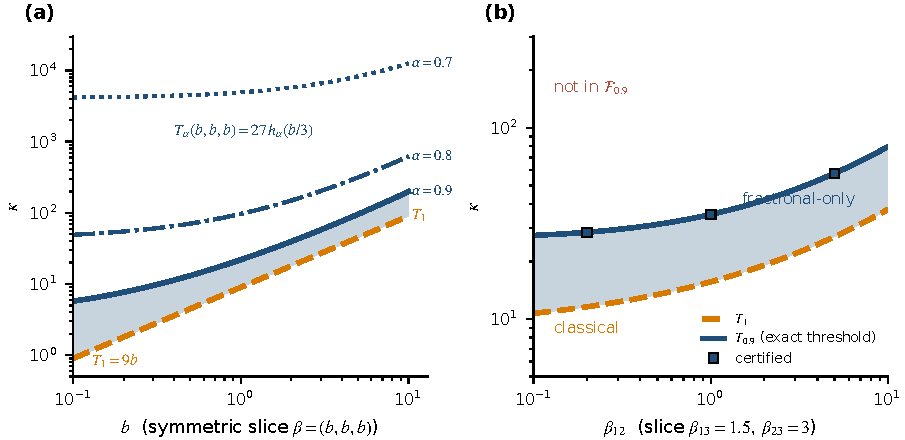
\includegraphics[width=0.92\textwidth]{fig03_threshold_geometry.pdf}
\caption{Exact positive-diagonal threshold geometry for real three-by-three matrices with strict-\(P(-A)\) principal minors. Orange: classical Cain boundary \(\kappa=T_1(\beta)\). Blue: fractional Matignon boundary \(\kappa=T_\alpha(\beta)\) for the indicated order. The open interval \(T_1<\kappa<T_\alpha\) is fractionally stable for every positive diagonal multiplier but not classically Hurwitz \(D\)-stable. The numerical markers corroborate exact formulas and are not substitutes for the all-diagonal proof.}
\label{fig:c10geometry}
\end{figure}

\subsection{Minimum Dimension for a Robust Fractional-Only Class}

The two-dimensional obstruction and the three-dimensional band give the dimension result.

\begin{Theorem}[minimum robust dimension]\label{thm:mindim}
For every \(0<\alpha<1\),
\begin{equation}
\boxed{
\min\left\{
n:
\operatorname{int}
\left(
\mathcal F_\alpha^{(n)}
\setminus
\mathcal D_H^{(n)}
\right)\ne\varnothing
\right\}=3.
}
\label{eq:min-dim}
\end{equation}
\end{Theorem}

\begin{proof}
Dimension one is trivial and Theorem~\ref{thm:2d} gives empty full-dimensional interior in dimension two. For \(2/3<\alpha<1\), Equation~\eqref{eq:strict-gap} makes the interval
\[
T_1(\beta)<\kappa<T_\alpha(\beta)
\]
nonempty for every positive \(\beta\); any strict interior point is stable under small full-matrix perturbations. For \(0<\alpha\le2/3\), choose any strict-\(P(-A)\) matrix violating Cain's inequality \(\kappa<T_1(\beta)\). Corollary~\ref{cor:fracband} then places it in \(\mathcal P_\alpha^{(3)}\), and strictness again gives a full-dimensional neighborhood.
\end{proof}
